\chapter{Illustrative Simulation Examples} \label{cha:practical-considerations}

In~\pref{cha:solution-approach}, we discussed the theoretical basis for shape-constraint P-splines and their ability to incorporate a priori domain knowledge into the fitting process by choice of the constraint term described by the mapping matrix $\vec{D}_c$ and the weighting matrix $\vec{V}_c$. We will now consider the practical application of these, as well as their limits in terms of data fitting and constraint fidelity  based on the example of peak behavior. We will evaluate the performance of shape-constraint P-splines using noisy data, see~\pref{sec:peak-behav-noisy}, and sparse data, see~\pref{sec:peak-behav-sparse}, and compare it to B-splines and P-splines. If not further stated, we will use equidistant knot placement throughout this section. Furthermore, we will discuss the effect of the constraint parameter $\lambda_c$, see~\pref{sec:lambda_c_sec}.

Throughout this chapter, we will use the function $f(x)$, i.e.

\begin{align} \label{eq:true-func-peak}
	f(x) = \exp\left(-\frac{(x - 0.35)^2}{0.1} \right)
\end{align}
% 
as underlying true function. The function is monotonically increasing up to the peak value at $x = 0.35$ and then monotonically decreasing.  

It is important to notice that the addition of the constraint term in~\pref{eq:OF-SCP-Final} further reduces the effective degree of freedom of the model, similar as for P-splines, resulting in a less flexible model. We therefore expect that the measured metric on the training data will be worse compared to a pure B-spline fit. Nevertheless, the metric of interest is the mean squared error MSE, see~\pref{eq:MSE-DEF}, on the validation data, i.e. the held out data that the model has not seen before. Supposing that the a priori domain knowledge reflects the true, underlying function behavior, we expect the measured error on the validation data to be lower than or equal to the error given by an optimal P-spline fit. Here, optimality is based on the optimal smoothing parameter $\lambda$ given by generalized cross-validation, see Section~\ref{subsubsec:Cross-validation}. This can be seen by recognizing the equivalence of the objective functions for P-splines, see~\pref{eq:P-spline-final-OF}, and shape-constraint P-splines, see~\pref{eq:OF-SCP-Final}, when the underlying B-spline fit does not violate the user-defined constraint, i.e. all $v_j=0$. Note this feature is one of the limits of shape-constraint P-splines, i.e. we cannot influence the model using this approach if no constraint violations are present. On the other hand, if the a priori domain knowledge reflects the underlying function, we can expect a far better generalization capability of the model compared to the B-spline fits, especially in situations of noisy or sparse data.



%%%%%%%%%%%%%%%%%%%%%%%%%%%%%%%%%%%%%%%%%%%%%%%%%%%%%%%%%%%%%%%%%%%%%%%%%%%%%%%%%%%%%%%%%%%%%%%%%%%%%%%%%%%%%%%%%%%%%%%%%%%%%%%%%
\section{Peak Constraint in Practice} \label{sec:peak-behav-noisy}

We will now utilize shape-constraint P-splines and the a priori domain knowledge of peak behavior to fit the data $\mathcal{D} = \{(x^{(i)}, y^{(i)}), \ i=1,2,\dots,n\}$. The data is artificially generated by random sampling of $n=200$ points $x^{(i)}$ in the interval $[0.1, 0.8]$. These are then used as input for the function $f(x)$ in~\pref{eq:true-func-peak} to generate the $y^{(i)}$ as

\begin{align}
	y^{(i)} = f(x^{(i)}) + \epsilon^{(i)},
\end{align}
%
with the Gaussian noise $\epsilon^{(i)}$ characterized by the mean $\mu = 0$ and the variance $\sigma^2 = 0.01$. We randomly split the data in a training set $\mathcal{D}_{\mathrm{train}}$ with 150 samples and a validation set $\mathcal{D}_{\mathrm{val}}$ with 50 samples.  For the validation set, we further generate the true validation set $\mathcal{D}_{\mathrm{val}, \mathrm{true}}$ for which we omit the Gaussian noise $\epsilon$ and therefore obtain the true function values given by the function in~\pref{eq:true-func-peak}. 

At first, we use $d=45$ B-spline basis functions of order $l=3$ to fit a B-spline to the training data $\mathcal{D}_{\mathrm{train}}$. Then, we fit a P-spline using the same configuration $d=45$ and $l=3$ with an optimal smoothness parameter $\lambda_{\mathrm{opt}} = 7.74$ determined by generalized cross-validation. Finally, we enforce the peak behavior with a shape-constraint P-spline, see~\pref{sec:SCP-splines}, with $d=45$ and $l=3$ as well as the optimal smoothness parameter $\lambda_{\mathrm{opt}}=7.74$ and the constraint parameter $\lambda_c=6000$ reflecting high trust in the a priori domain knowledge. The various fits and the full data $\mathcal D$ are shown in~\pref{fig:test-func-peak-fit}. The mean squared errors MSE, see~\pref{eq:MSE-DEF}, on the validation data, as well as on the true, underlying function in~\pref{eq:true-func-peak}, are given in~\pref{tab:test-func-peak-mses}.


\begin{figure}[H]
	\centering
	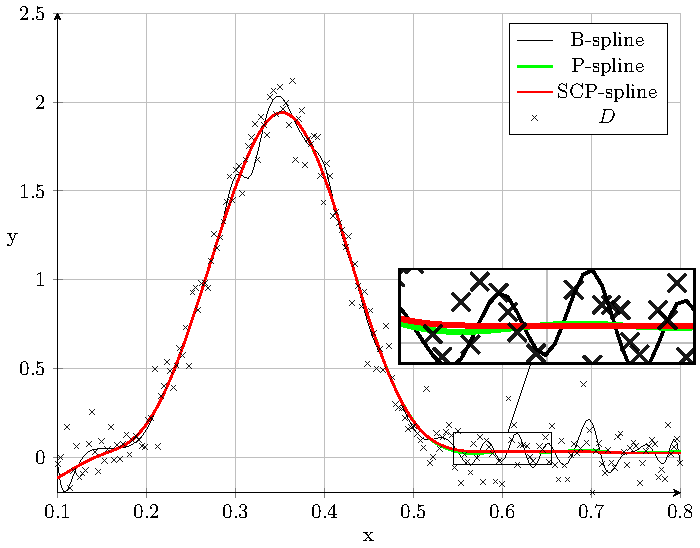
\includegraphics{graphics/pgfplots/cha4/exp-peak.pdf}
	\caption{B-spline, P-spline and SCP-spline fit for the data $\mathcal{D}$.}
	\label{fig:test-func-peak-fit}
\end{figure}
%
The B-spline, as black curve in~\pref{fig:test-func-peak-fit}, captures the basic shape of the true function, but the flexibility of the B-spline, due to the high number of B-spline basis functions, leads to a wiggly estimate especially for the almost constant part. This violates the peak behavior of the true function which is being monotonically decreasing for $x \in [0.35, 0.8]$. For the P-spline (green), this problem relaxes due to the smoothing aspect of the penalty term but does not completely vanish, as seen in the magnified part in~\pref{fig:test-func-peak-fit}. Note that the additional smoothness penalty given by the P-spline already fits the data almost perfectly with respect to a smooth result. The SCP-spline estimate gives almost identical results as the P-spline as it adjusts only the parts of the P-spline, which violate the peak constraint. It may be seen as "fine-tuning" of the fit using the a priori domain knowledge. Hence, it is the best solution here based on a visual interpretation of the a priori knowledge.

\begin{table}[H]
	\begin{center}
		\pgfplotstabletypeset[
		col sep=comma,
		columns/Model/.style={string type},
		columns/MSEVal/.style={column name={$\text{MSE}_{\mathcal{D}_{\mathrm{val}}}$}},
		columns/MSEValTrueFunction/.style={column name={$\text{MSE}_{\mathcal{D}_{\mathrm{val},\mathrm{true}}}$}},
		every head row/.style={before row=\toprule[1pt] \toprule,after row=\midrule[2pt]},
		every last row/.style={after row=\bottomrule \bottomrule},
		every nth row={1}{before row=\midrule},
		]{graphics/data/cha4/peak_example/mse.csv}
	\end{center}
	\caption{Mean squared errors on the validation set $\mathcal{D}_{\text{val}}$ and the true validation set $\mathcal{D}_{\mathrm{val}, \mathrm{true}}$}
	\label{tab:test-func-peak-mses}
\end{table}
%
The mean square errors $\mathrm{MSE}_{\mathcal{D}_{\mathrm{val}}}$, see~\pref{eq:MSE-DEF}, on the noisy validation data $\mathcal{D}_{\mathrm{val}}$ in~\pref{tab:test-func-peak-mses} for P-spline and SCP-spline are almost identical and do not show a favorable model. Comparing the various models with the true, underlying function by calculating $\text{MSE}_{D_{\mathrm{val},\mathrm{true}}}$, i.e. the mean squared error on the true function values, leads to the assessment that the SCP-spline is the more accurate model with regard to the a priori knowledge. This also coincides with the graphs in~\pref{fig:test-func-peak-fit}. Hence, the incorporation of a priori domain knowledge via shape-constraints improves the generalization capability measured by the mean squared error on the true function values in our example. 
%%%%%%%%%%%%%%%%%%%%%%%%%%%%%%%%%%%%%%%%%%%%%%%%%%%%%%%%%%%%%%%%%%%%%%%%%%%%%%%%%%%%%%%%%%%%%%%%%%%%%%%%%%%%%%%%%%%%%%%%%%%%%%%%%

\section{Peak Constraint and Sparse Data} \label{sec:peak-behav-sparse}

We will now examine the behavior of B-, P- and SCP-splines for sparse data, i.e. few data and unevenly distributed, sampled from the function in~\pref{eq:true-func-peak}. The data set $\mathcal{D}$ now contains 70 data points distributed in a way that there is only few data in the peak region, i.e. for $x \in [0.2, 0.5]$. In this region, we have only 10 data points. We perform an random train-validation split of the data in $\mathcal{D}$, i.e. the training data $\mathcal{D}_{\text{train}}$ consists of 52 points and the validation data $\mathcal{D}_{\text{val}}$ consists of 18 points. For the validation set, we again generate the true validation set $\mathcal{D}_{\mathrm{val}, \mathrm{true}}$ for which we omit the Gaussian noise $\epsilon$.


We follow the same approach as above, i.e. fit a B-spline, perform generalized cross-validation to determine the optimal P-spline and finally apply the shape-constraint to enforce the peak behavior. The small data set indicates that a different, not equidistant knot placement may be helpful. Hence, we carry out 2 experiments, one with equidistant knot placement and the other with quantile-based knot placement, see Section~\ref{subsec:b-splines} for further information on quantile-based knot placement. We use $d=25$ B-spline basis functions of order $l=3$. The optimal smoothness parameter was given as $\lambda_{\mathrm{opt}} = 0.00657$ for the equidistant fit and $\lambda_{\mathrm{opt}} = 0.00215$ for the quantile-based fit determined by generalized cross-validation. The constraint parameter $\lambda_c$ was set to $\lambda_c=1000$ for both fits, reflecting high trust in the a priori domain knowledge. \pref{fig:sparse-example-equidistant} shows the resulting fits with equidistant knot placement and~\pref{fig:sparse-example-quantile} with quantile-based knot placement.


\begin{figure}[H]
	\centering
	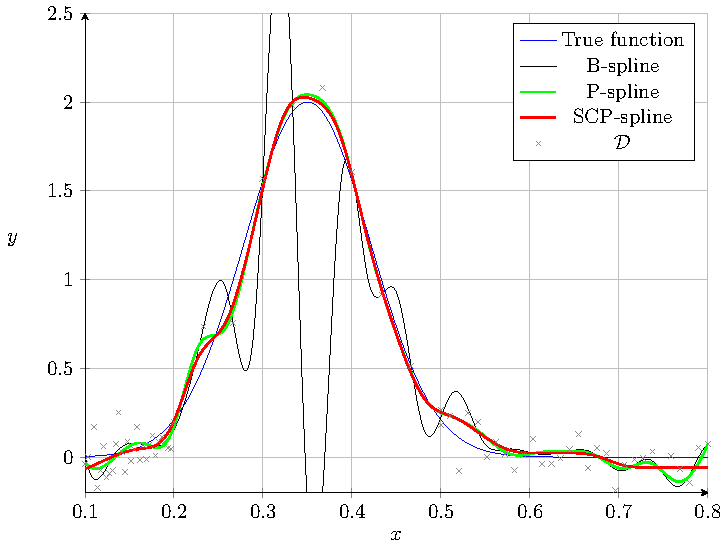
\includegraphics{graphics/pgfplots/cha4/exp-sparse-equidistant.pdf}
	\caption{Equidistant B-spline, P-spline and SCP-spline fit for sparse data $\mathcal{D}$.}
	\label{fig:sparse-example-equidistant}
\end{figure}

The B-spline (black) in~\pref{fig:sparse-example-equidistant} shows the problem of equidistant knot placement in sparse data situations. The estimate becomes very wiggly in the region of few data, similar to polynomial fits with a high polynomial degree. Nevertheless, utilizing the regularization through the additional smoothness penalty in P-splines, the estimate (green) becomes smoother and reflects the true function quite well. The shape-constraint P-spline (red) further improves the quality of the fit, which can be seen by a comparison of the mean squared errors MSE, see~\pref{eq:MSE-DEF}, in~\pref{tab:sparse-example-equidistant}. 

\begin{table}[H]
	\begin{center}
		\pgfplotstabletypeset[
		col sep=comma,
		columns/Model/.style={string type},
		columns/MSEVal/.style={column name={$\text{MSE}_{\mathcal{D}_{\mathrm{val}}}$}},
		columns/MSEValTrueFunction/.style={column name={$\text{MSE}_{\mathcal{D}_{\mathrm{val},\mathrm{true}}}$}},
		every head row/.style={before row=\toprule[1pt] \toprule,after row=\midrule[2pt]},
		every last row/.style={after row=\bottomrule \bottomrule},
		every nth row={1}{before row=\midrule},
		]{graphics/data/cha4/sparse_example/mse-e.csv}
	\end{center}
	\caption{Mean squared errors on the validation set $\mathcal{D}_{\mathrm{val}}$ and the true validation set $\mathcal{D}_{\mathrm{val},\mathrm{true}}$ for equidistant knot placement.}
	\label{tab:sparse-example-equidistant}
\end{table}


\begin{figure}[H]
	\centering
	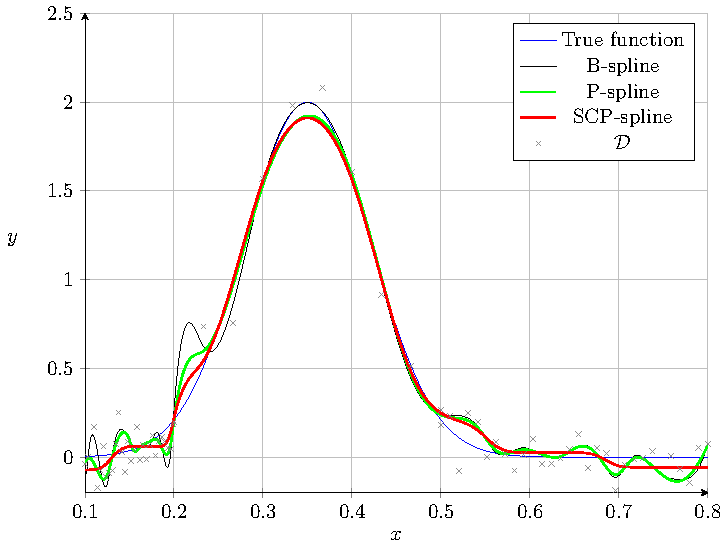
\includegraphics{graphics/pgfplots/cha4/exp-sparse-quantile.pdf}
	\caption{Quantile-based B-spline, P-spline and SCP-spline fit for sparse data $\mathcal{D}$.}
	\label{fig:sparse-example-quantile}
\end{figure}

The quantile-based B-spline (black) in~\pref{fig:sparse-example-quantile} shows some interesting features. At first, it fits the peak surprisingly well despite the small sample size in this area. This is due to the inherent smoothing aspect of quantile-based knot placement in regions of small sample size, see~\ref{subsec:b-splines}. Further, we see the flexibility of the B-spline in the regions with more data, i.e. $x\in[0.1,0.2]$ and $x \in [0.5,0.8]$, where it clearly reproduces the noise part instead of the true function. Hence, quantile-based knot placement may lead to partial overfitting, i.e. overfitting of the estimate only on a part of the input space. The P-spline (green) does not resolve this problem as the estimates (black and green) overlap almost everywhere. The reason for this effect is based on the approximation of the smoothness penalty term~\pref{eq:p-spline-approx-deriv} by means of the second-order finite difference~\pref{eq:wiggliness-finite-diff-approx}, which is valid for equidistant knot placement. However, a weighting arises for quantile-based knot placement. Nevertheless, including additional regularization through the shape-constraint leads to an estimate which is smooth, follows the a priori domain knowledge and generalizes better, also demonstrated by the comparison of $\text{MSE}_{D_{\mathrm{val}}}$ and $\text{MSE}_{D_{\mathrm{val}, \mathrm{true}}}$ in~\pref{tab:sparse-example-quantile}.


\begin{table}[H]
	\begin{center}
		\pgfplotstabletypeset[
		col sep=comma,
		columns/Model/.style={string type},
		columns/MSEVal/.style={column name={$\text{MSE}_{\mathcal{D}_{\mathrm{val}}}$}},
		columns/MSEValTrueFunction/.style={column name={$\text{MSE}_{\mathcal{D}_{\mathrm{val},\mathrm{true}}}$}},
		every head row/.style={before row=\toprule[1pt] \toprule,after row=\midrule[2pt]},
		every last row/.style={after row=\bottomrule \bottomrule},
		every nth row={1}{before row=\midrule},
		]{graphics/data/cha4/sparse_example/mse-q.csv}
	\end{center}
	\caption{Mean squared errors on the validation set $\mathcal{D}_{\mathrm{val}}$ and the true validation set $\mathcal{D}_{\mathrm{val},\mathrm{true}}$ for quantile-based knot placement.}
	\label{tab:sparse-example-quantile}
\end{table}
%
To summarize, we can conclude that equidistant knot placement is superior to quantile-based knot placement in this example as it yields lower mean squared errors MSE on the validation set $\mathcal{D}_{\mathrm{val}}$ and on the true validation set $\mathcal{D}_{\mathrm{val}, \mathrm{true}}$, seen in~\pref{tab:sparse-example-equidistant} and~\pref{tab:sparse-example-quantile}.
%%%%%%%%%%%%%%%%%%%%%%%%%%%%%%%%%%%%%%%%%%%%%%%%%%%%%%%%%%%%%%%%%%%%%%%%%%%%%%%%%%%%%%%%%%%%%%%%%%%%%%%%%%%%%%%%%%%%%%%%%%%%%%%%%

\section{The Effect of the Constraint Parameter $\lambda_c$} \label{sec:lambda_c_sec}

We will now discuss the effect of the constraint parameter $\lambda_c$. As noted in~\pref{sec:peak-behav-noisy}, the shape-constraint acts as "fine-tuning" of the estimate according to the a priori domain knowledge, i.e. it only changes the estimate at locations where it violates the user-defined shape constraint. We use the constraint parameter $\lambda_c$ as a measure of trust in the a priori domain knowledge, such that high trust is reflected by high values of $\lambda_c$. To show this in practice, we use the data $\mathcal{D}$ given in~\pref{sec:peak-behav-noisy} and fit shape-constraint P-splines using various values of the parameter $\lambda_c$. The results are show in~\pref{fig:example-lambdas}. Since most constraint violations are present for larger $x > 0.55$, we focus on this part of the data. 

\begin{figure}[H]
	\centering
	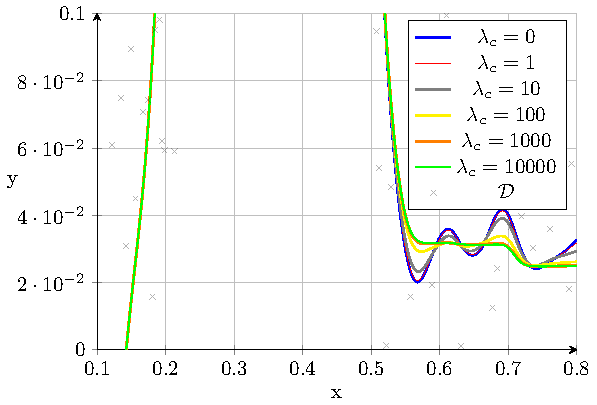
\includegraphics{graphics/pgfplots/cha4/exp-lambdas.pdf}
	\caption{SCP-splines for different $\lambda_c$ for data $\mathcal{D}$.}
	\label{fig:example-lambdas}
\end{figure}	

In~\pref{fig:example-lambdas}, we clearly see that with increasing $\lambda_c$ we enforce the a priori domain knowledge. For small $\lambda_c \le 10$, the estimates (blue, red and gray) violate the constraint qualitatively quite strong. Medium values of $\lambda_c = 100$ already produce an estimate (yellow) that follows the constraint far better, but not optimally. High values of $\lambda_c \ge 1000$ enforce the a priori domain knowledge, as seen by the orange and the green estimate. Nevertheless, quantitatively small violations of the a priori domain knowledge are possible even for this values of the constraint parameters. 
